% use the standard article class with 12pt font
\documentclass[12pt]{article}

% load a minimal set of packages packages
\usepackage{fullpage}
\usepackage{setspace}
\usepackage{graphicx}
\usepackage{natbib}
\usepackage{amsmath}
\usepackage{amsfonts}
\usepackage{amssymb}
\usepackage{hyperref}
\bibpunct{(}{)}{;}{a}{}{,}

% set custom paragraph spacing 
\parskip=0pt
\parindent=20pt

% create footnote command so that my name
% has an asterisk rather than a one.
\long\def\symbolfootnote[#1]#2{\begingroup%
\def\thefootnote{\fnsymbol{footnote}}\footnote[#1]{#2}\endgroup}

% set up references. eliminate distracting boxes and colors.
\hypersetup{
  colorlinks=true, % false: boxed links; true: colored links
  linkcolor=black, % color of internal links
  citecolor=black, % color of links to bibliography
  filecolor=blue, % color of file links
  urlcolor=blue % color of external links
}

% begin the document
\begin{document}

% insert title manually (personal preference)
\begin{center}
{\LARGE \textbf{Party Heterogeneity}}\\\vspace{2mm}
{ \textbf{Variation in the Variance Across Space and Time}}\symbolfootnote[1]{Thanks to everyone who helped me.}

\vspace{5mm}

Carlisle Rainey\symbolfootnote[2]{Carlisle Rainey is Assistant Professor of Political Science, Texas A\&M University, 2010 Allen Building, College Station, TX, 77843 (\href{mailto:crainey@tamu.edu}{crainey@tamu.edu}).}
\end{center}

\vspace{5mm}

% abstract
{\centerline{\textbf{Abstract}}}
\begin{quote}
\noindent Put the abstract here...
\end{quote}

% remove page number from first page
\thispagestyle{empty}

% start main text
\doublespace

Start the introduction here...

\section*{A Heading}

Continue here...

\subsection*{A Sub-Heading}

Continue...

\section*{See LaTeX at Work}

Below, I use LaTeX syntax to automatically include references, create mathematical equations, incude and refence the figure.

\cite{shor-mccarty-2011} and \cite{shor-berry-mccarty-2010} develop the statistical theory to estimate the ideology of state legislators along a single left-right dimmension. Using data from \cite{shor-2018-data}, I calculate the standard deviation of the legislators' ideologies for each state-party-year. Figure \ref{fig:sds} shows these standard deviations, calculated as $\sqrt{\frac{1}{N-1} \sum_{i=1}^N (x_i - \overline{x})^2}$, where $i$ indexes the legislators in each state-party-year and $N$ represents the total number of legislators in the state-party-year.

% add the figure
\begin{figure}[h!]
\begin{center}
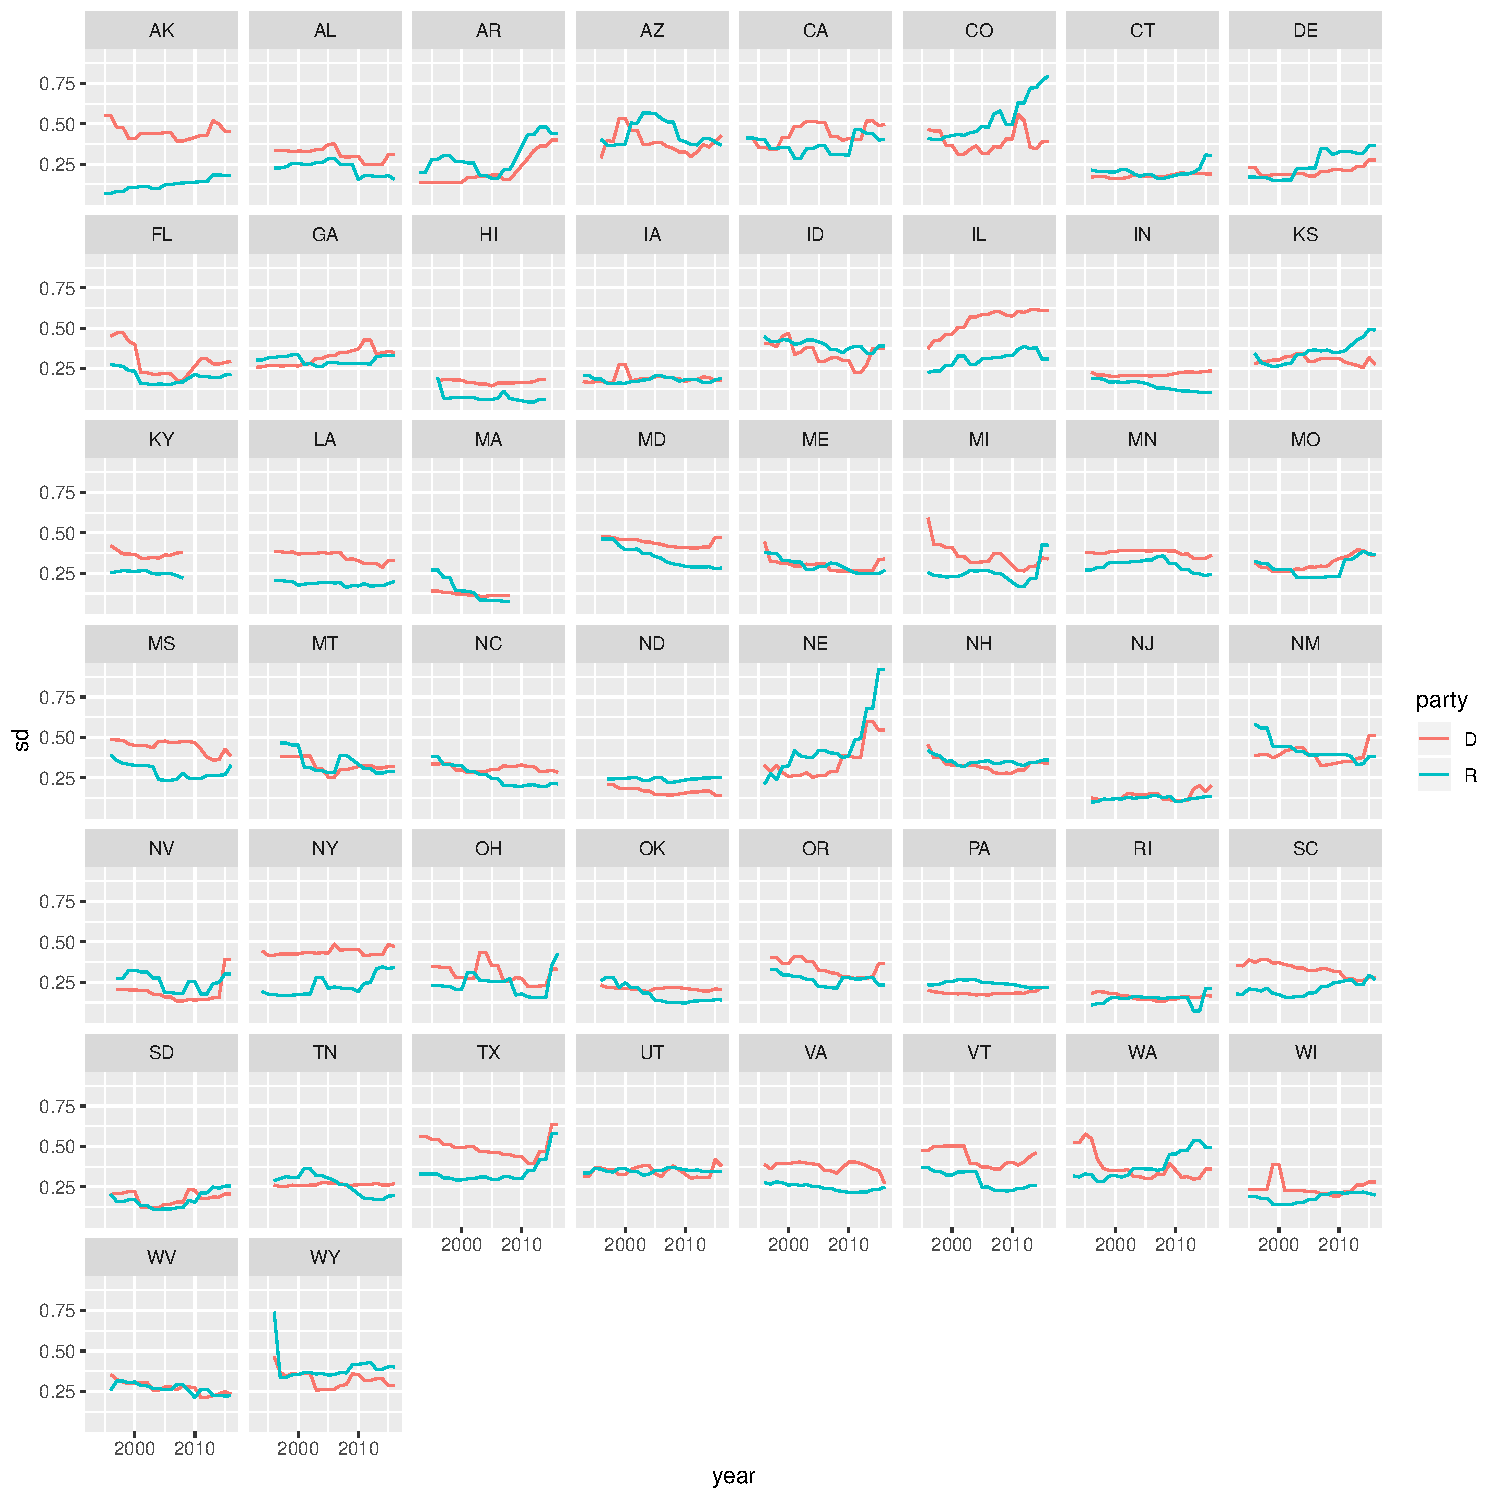
\includegraphics[width = \textwidth]{figs/sds.pdf}
\caption{This figure shows the standard deviations of each state-party-year in the data from \cite{shor-2018-data}.}\label{fig:sds}
\end{center}
\end{figure}

\singlespace 
\bibliographystyle{apsr-fs}
\bibliography{bibliography}

\end{document}

















